\chapter{Optimierung auf Basis der ausgewerteten Testdaten}
Für die in Kapitel \ref{sec:analysisTests} aufgedeckten Probleme werden in diesem Abschnitt Lösungen erarbeitet und umgesetzt. Abschließend wird ein vergleichender Kontrolltest durchgeführt, um zu verifizieren, ob die unternommenen Veränderungen wirklich den gewünschten Effekt auf den Nutzer haben.\par
\section{Design der Lösungen} \label{sec:optiDesign}
Das erste zu behandelnde Problem ist die die Filterauswahl in der Sidebar. Hier muss verdeutlicht werden, dass die Elemente angeklickt werden können und sowohl das \textbf{-} -Icon, das nur als Hover-Effekt angezeigt wird, als auch der Text zu einer Einheit gehören. Zwar unterstützt die orangefarbene Hinterlegung des gesamten Elementes während des Hoverns bei der Identifizierung als ein einzelnes Objekt, aber die Animation, mit der das \textbf{-} -Symbol erscheint, wirkt dem entgegen (Gesetz des gemeinsamen Schicksals). Eine einfache Möglichkeit, zu signalisieren, dass das gesamte Element angeklickt werden kann, ist das Hinzufügen des typischen Hand-Cursors für Elemente, die angeklickt werden können.\par
%Für den Kopfzeilenfilter der Ergebnistabelle kann eine ähnliche Suchfunktion umgesetzt werden, wie für die Galerie. Eine Freitexteingabe, die ein Scrollen zum gesuchten Element hervorruft, kann hier genauso dabei unterstützen, das richtige Element zu finden. Das gleiche Konzept kann auch für die Ergebnistabelle selbst übernommen werden. In diesem Fall würde das primäre Attribut, die Benennung, für die Suche ausschlaggebend sein.\par
Während der Lesemodus aktiv war, versuchte ein Nutzer die Galerie im Hintergrund zu bedienen. Um dies zu unterbinden und deutlich zu machen, dass die Bedienelemente im Hintergrund derzeit nicht verwendbar sind, kann entweder die Transparenz des vordergründigen Lesemodus verringert werden oder alternativ über die hintergründigen Komponenten ein Effekt gelegt werden, der die Darstellung \enquote{verwischt}. Dieser Effekt nennt sich \textit{Blur}-Effekt. Dadurch sind die Elemente noch immer sichtbar, aber durch die verschwommenen Konturen wird deutlich, dass sie derzeit nicht für eine Bedienung geeignet sind. Aufgrund der Ästhetik ist die zweite Variante die bevorzugte Alternative.\par
Das \ding{58}-Icon in der Navigationsleiste bereitete auf zweierlei Weisen Probleme. Zunächst wurde es nicht als klickbares Element wahrgenommen und nachdem es doch gefunden wurde, hatten einige Nutzer das Problem, die Schaltfläche mit dem Mausklick zu treffen. Um das erste Problem zu lösen, muss die Aufmerksamkeit des Benutzers bewusst auf das neu erschienene Element gelenkt werden. Dies kann durch eine Animation geschehen, die abläuft, sobald das Symbol angezeigt wird. Ein \textit{Glow}-Effekt (kurzes Aufblinken) sollte diesen Zweck erfüllen. Damit die Schaltfläche besser bedient werden kann, kann der Bereich, in dem der Klick dem \ding{58}-Icon gilt, vergrößert werden. So werden leicht verfehlte Klicks dennoch für das richtige Element registriert.\par
Der Eintrag \textit{[Alle Werte]} in der Multi-Level-Liste sollte sich, gemäß des Gesetzes der Prägnanz, deutlicher von dem Rest der Einträge abheben, damit es eher erkannt und nicht als Teil der möglichen Werte gesehen wird. Ein einfaches Fettdrucken des Textes sollte für diesen Zweck genügen. Außerdem kann der Eintrag entfernt werden, sobald kein weiteres Element in der Liste ist und einem Infotext weichen, durch den die leere Liste erklärt wird.\par
Für den Vollbildmodus kann der Hotkey \enquote{F11} bedenkenlos hinzugefügt werden. Dies muss jedoch auf andere Weise geschehen als mit dem bisherigen Mnemonic-Konzept, das bewusst nur sichtbare Elemente unterstützt. Die Vollbildfunktion ist nicht immer sichtbar.\par
Sämtliche Ergebnistabellen und -listen benötigen einen Hinweistext, der angezeigt wird, wenn kein Element in diesen dargestellt wird, um dem Punkt \textit{\enquote{Gibt es Unterstützung bei Fehlern?}} der Usability-Heuristik von Nielsen und Molich zu entsprechen.\par
Die Subnavigation in der Detailansicht ist für den Anwender nicht eindeutig erkennbar. Unter Umständen Ist der orangefarbene Text des selektierten Unterpunktes schwerer zu erkennen als das schwarz des nicht-selektierten Unterpunktes. Ein kurzer Blick zu diesen Elementen reicht nicht aus, um den selektierten Punkt auszumachen, daher sollte der Text durch Fettdrucken prägnanter dargestellt werden.\par
% Hilfetexte?
\section{Umsetzung} \label{sec:optiImplementation}
\heading{Mauszeiger Filterauswahl}
Der Mauszeiger auf den einzelnen Elementen der Filterselektion ließ sich umsetzen, indem der Cursor innerhalb der \textit{\#{}updateItem}-Methode der verwendeten Listenzelle gesetzt wird. Hierbei muss darauf geachtet werden, dass der Cursor gesetzt wird, wenn die Listenzelle einen Text beinhaltet und zurückgesetzt wird, wenn der Text leer ist. Die Besonderheit der Listenzelle in JavaFX ist die Wiederverwendung dieser. Anstatt für jedes Item der Liste eine neue Listenzelle zu erzeugen werden die Zellenobjekte wiederverwendet und nur die Eigenschaften und der Inhalt dieser aktualisiert.\par
\heading{Lesemodus}
Um den Blur-Effekt für den Hintergrund des Lesemodus zu setzen, wird die Methode \textit{\#{}setEffect} verwendet, die auf jeder JavaFX-Komponente verfügbar ist. Als Übergabeparameter dient ein sogenanter BoxBlur-Effekt, der vorab konfiguriert wird. Wird der Effekt auf dem Wurzelknoten des ursprünglichen Inhaltes gesetzt, der mit Öffnen des Lesemodus in der Hintergrund rückt, wird die Ansicht des Hintergrundes verschwommen und der Fokus auf die vordergründigen Objekte gelenkt. Die Wahrscheinlichkeit, dass ein Anwender versucht, Bedienelemente zu nutzen, die sich im Hintergrund befinden, wird dadurch stark verringert.\par
\begin{figure}[H] 
	\centering
	\subfloat[Ohne Blur] {
		 
\includegraphics[width=0.45\textwidth]{grafiken/readmode_no_blur.png}
	}
	\hspace{1.0em}
	\subfloat[Mit Blur] {
		 
\includegraphics[width=0.45\textwidth]{grafiken/readmode_blur.png}
	}
	\caption{Beispiel: Blur-Effekt im Lesemodus}
	\label{fig:blurGallery}
\end{figure}
\heading{Erweiterte Funktionen der Navigationsleiste}
Auch für das Hervorheben des \ding{58}-Icons in der Navigationsleiste kommt ebenfalls ein Effekt zum Tragen. Allerdings wird hier ein sogenannter \textit{DropShadow} verwendet. Die Eigenschaften des Effektes sind so konfiguriert, dass der \textit{DropShadow} standardmäßig nicht sichtbar ist, da die Größe 0 x 0 Pixel beträgt. Wird zu einem anderen Menüpunkt gesprungen, der erweiterte Funktionen unterstützt, wird mit Erscheinen des \ding{58}-Icons der Effekt im Rahmen einer Animation so verändert, dass sich die Größe von anfänglich 0 Pixeln gleichmäßig in alle Richtungen vergrößert. Die Animation ist so eingestellt, dass sich der Effekt 1 Sekunde lang ausbreitet und mit Abschluss dieser innerhalb einer weiteren Sekunde wieder zusammenzieht. Das Zusammenziehen wird allerdings durch das Animieren eines anderen Properties gelöst. Der \textit{DropShadow} besitzt ein \textit{Spread}- Property, das die Ausbreitung des Effektes bestimmt. Sobald dieser Wert 0 erreicht, ist die Animation abgeschlossen und alle Werte werden auf ihren Ausgangszustand zurückgesetzt. Durch das Animieren der beiden unterschiedlichen Effekt-Eigenschaften wird die Aufmerksamkeit des Anwenders auf attraktive Weise auf das neu erschienene Symbol gelenkt.\par
\begin{figure}[H]
 \centering
 
\includegraphics[width=0.75\textwidth]{grafiken/glow_animation.png}
 \caption{Glow Animation}
 \label{fig:glowAnimation}
\end{figure}
\heading{Spezialeintrag \textit{[Alle Werte]}}
Das Fettdrucken des Eintrages \textit{[Alle Werte]} in der Multi-Level-Liste konnte durch eine simple Fallunterscheidung innerhalb der angepassten Listenzellen-Klasse gelöst werden. Bei Ausführung der \textit{\#{}updateItem}-Funktion wird überprüft, ob das Element, das ab sofort in der Listenzelle angezeigt werden soll in der Werteliste enthalten ist, die der JavaFX-ListView zugrunde liegt. Ist dies nicht der Fall, handelt es sich um das nachträglich hinzugefügte Spezialelement \textit{[Alle Werte]}. In diesem Falle wird der Listenzelle eine CSS-Klasse zugewiesen, durch die jeglicher in der Zelle enthaltener Text fett dargestellt wird. Das Element grenzt sich so deutlich von den übrigen Elementen ab.\par
\begin{figure}[H]
 \centering
 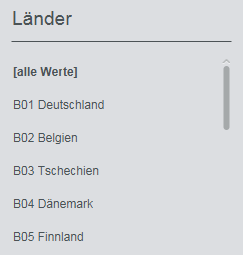
\includegraphics[width=0.35\textwidth]{grafiken/mll_Werte.png}
 \caption{Multi-Level-Liste Spezialeintrag}
 \label{fig:mllSpecialValue}
\end{figure}
\heading{Schnelltaste für Vollbildmodus}
Das Aktivieren des Lesemodus ist nun auch per Schnelltaste \textit{F11} möglich. Dazu wird die Tastatureingabe über das bereits vorgestellte Konzept der globalen Eingabeerkennung (vgl. Kap. \ref{sec:interactionImplementation}) verarbeitet. Der Vollbildmodus wird nur aktiviert, wenn der korrespondierende Menüpunkt auch aktiviert ist und die gedrückte Taste der \textit{F11} Taste entspricht. In diesem Fall wird das Event konsumiert - andere, im Szenegraphen tiefer liegende Knoten, die ein solches Event ggf. behandeln würden, werden in diesem Falle nicht von dem Event benachrichtigt.\par
\heading{Hilfetext leere Liste/ Tabelle}
Der Hilfetext für leere Tabellen und Listen wird durch ein Label repräsentiert, dessen Sichtbarkeit von der Länge der jeweiligen Liste oder Tabelle abhängt. Sobald kein Element mehr vorhanden ist, wird das Label sichtbar. Der Text liegt also immer über der entsprechenden Ansicht, wird jedoch nur in der speziellen Situation angezeigt, dass die Tabelle oder Liste leer ist. Die Position des Textes entspricht der eigentlichen Position der ersten Zeile. In der Multi-Level-Liste wird zudem der Spezialeintrag \textit{[Alle Werte]} entfernt, wenn der Hilfetext dargestellt werden soll.\par
\begin{figure}[H]
 \centering
 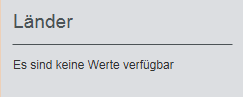
\includegraphics[width=0.35\textwidth]{grafiken/mll_no_values.png}
 \caption{Multi-Level-Liste Infotext}
 \label{fig:mllNoValues}
\end{figure}
\heading{Subnavigation Detailansicht}
Damit das ausgewählte Element in der Subnavigation der Detailansicht deutlicher hervorgehoben wird, wird der Text fett gedruckt. Die Funktion wird über eine CSS-Pseudoklasse realisiert, die auf dem Label des selektierten Elementes gesetzt und bei Änderung aktualisiert wird. Eine CSS-Pseudoklasse wird in einer CSS-Datei durch einen Bezeichner angesprochen, der durch einen Doppelpunkt vom Rest des CSS-Selektors abgetrennt wird. Die für das Label neu definierte Pseudoklasse namens \enquote{selected} wird immer dem Punkt zugewiesen, der gerade angewählt ist. Der CSS-Selektor trifft also immer auf das Label zu, das den \enquote{selektiert}-Status besitzt und stellt dessen Text hervorgehoben dar.\par
\begin{figure}[H]
 \centering
 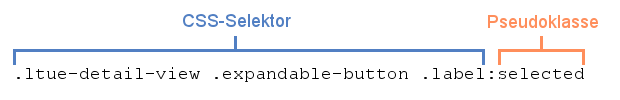
\includegraphics[width=0.9\textwidth]{grafiken/pseudoklasse.png}
 \caption{CSS Pseudoklasse}
 \label{fig:cssPseudoclass}
\end{figure}
Eine Pseudoklasse wird in JavaFX durch eine Ableitung der abstrakten Klasse \textit{Pseudoclass} ermöglicht. Die einzige Information, die durch diese Ableitung zur Verfügung gestellt wird, ist der Name der Pseudoklasse. Durch den Aufruf \textit{Node\#{}pseudoClassStateChanged(Pseudoclass, boolean)} kann der Status der Pseudoklasse verändert werden. Die Pseudoklasse muss der Komponente dazu nicht explizit hinzugefügt werden.\par
\begin{figure}[H]
 \centering
 
\includegraphics[width=0.5\textwidth]{grafiken/detailPage_bold.png}
 \caption{Detailansicht Überschrift}
 \label{fig:detailPageBold}
\end{figure}
\section{Vereinfachte Kontrolltests} \label{sec:optiQuality}
Zur Verifikation, dass die auf Basis der Nutzertests umgesetzten Funktionen eingänglich sind und tatsächlich eine Optimierung darstellen, wird ein vereinfachter, formloser A/B-Test durchgeführt. Im Rahmen des Testes werden die Funktionen in ihrer bisherigen Form und in ihrer Form nach der Implementierung durch einige Testkandidaten verglichen. Die Kandidaten müssen sich jeweils für die von ihnen bevorzugte Lösung entscheiden. Der Vergleich kann nur bei Funktionen durchgeführt werden, die eine Änderung am User-Interface erforderlich machten. Die Kandidaten sind zum Teil diejenigen, die auch an dem Formalen Usability-Test teilgenommen haben, als auch unbefangene Testpersonen. Insgesamt werden 6 Personen befragt.\par
\heading{Blur-Effekt im Lesemodus}
Der Effekt auf dem Hintergrund des Lesemodus wird von fast allen Kandidaten als positiv empfunden, da der Fokus auf diese Weise eher auf die vordergründigen Objekte gelenkt wird. Das Ziel der Verbesserung, den Hintergrund nicht mehr als bedienbar erscheinen zu lassen, wurde erreicht.
\heading{Erweiterte Funktionen der Navigationsleiste}
Nach Meinung der befragten Personen ist die Animation ansehnlich und trägt dazu bei, die Aufmerksamkeit auf das \ding{58}-Symbol zu lenken. Es wurden allerdings Bedenken geäußert, dass die Animation unter Umständen nicht deutlich genug sein könnte. Eine auffälligere Animation würde von erfahrenen Nutzern jedoch möglicherweise als störend empfunden werden.\par
\heading{Hilfetexte leere Tabelle/ Liste}
Die Hilfetexte bei leeren Tabellen oder Listen wurden ausnahmslos als vorteilhafte Neuerung empfunden.
\heading{Spezialeintrag \textit{[Alle Werte]}}
Bei der Funktion \textit{[Alle Werte]} in der Multi-Level-Liste gab es mehr Diskrepanz als bei den anderen umgesetzten Funktionen. Hier sind nur zwei Drittel der Befragten davon überzeugt, dass die Hervorhebung notwendig ist. Das verbleibende Drittel ist der Meinung, dass alleine durch den Text und die umschließenden viereckigen Klammern ausreichend Unterschied zu den übrigen Einträgen geschaffen wird. Obwohl die Notwendigkeit der Hervorhebung durch einige Testkandidaten angezweifelt wird, wird die Funktion nicht als nachteilig empfunden.\par
\heading{Subnavigation Detailansicht}
Auch hier waren sich die Testkandidaten uneinig, ob es nötig ist, den selektierten Punkt fettgedruckt darzustellen. 4 der 6 Personen jedoch bevorzugten die fettgedruckte Variante. Die Begründung lautete, dass ansonsten der schwarzfarbige, nicht selektierte Menüpunkt auf dem hell-orangefarbenen Hintergrund deutlicher hervorsteche als der dunkel-orangefarbene Text.\par